\chapter{Apprentissage profond et détection d'objet: Concepts et algorithmes}
\markboth{Apprentissage profond et détection d'objet: Concepts et algorithmes}{}
\section{Introduction}
%%%%%%%%%\Ajouter l'architecture YOLOV8%%%%%%%%%%%%%%%%
Au cours des vingt dernières années, des technologies avancées telles que l'intelligence artificielle, l'apprentissage automatique et la vision par ordinateur sont passées de la recherche et du développement à des environnements commerciaux et grand public.
\\
L'adaptation commerciale a vu des chaînes de montage automatisées de production de robots, des systèmes de guidage automatisés de véhicules et l'analyse d'images capturées à distance pour faciliter les stratégies d'inspection visuelle automatisées. En conséquence, les applications de vision par ordinateur et d'apprentissage automatique font partie des sujets techniques les plus séduisants et les plus fascinants de nos jours. Et la plupart des entreprises modernes de l'industrie technologique et des start-ups technologiques ambitieuses se précipitent pour profiter des avantages de ces technologies de pointe.
\\
Les progrès de l'apprentissage automatique et de la vision par ordinateur ont eu un impact significatif sur divers secteurs industriels, y compris la gestion des parkings. Grâce à ces technologies avancées, les machines sont capables d'apprendre à partir de données et de traiter diverses informations, offrant ainsi de nouvelles possibilités pour optimiser les performances de la gestion des parkings.
\\
Dans ce chapitre, nous explorons en détail l'apprentissage profond et ses différentes architectures. Nous fournissons également un aperçu des principaux algorithmes développés spécifiquement pour la détection d'objets. Enfin, nous présentons différentes mesures de performance essentielles pour évaluer les modèles de classification et les détecteurs d'objet.

\section{Intelligence artificielle }
L'intelligence artificielle (IA) fait référence à la théorie et au développement de systèmes informatiques capables d'effectuer des tâches qui nécessitent généralement l'intelligence humaine, telles que la perception visuelle, la reconnaissance de la parole, la prise de décision et la traduction entre les langues et bien d'autres. Le terme est fréquemment utilisé pour décrire des systèmes conçus pour imiter les processus intellectuels humains, tels que la capacité de raisonner d'apprendre, de percevoir, de comprendre et d'interagir avec l'environnement de manière autonome \cite{Questceq75}.
\\
C'est un domaine domaine interdisciplinaire  qui regroupe plusieurs sous-domaines, notamment l'apprentissage automatique et la vision par ordinateur.

\section{Apprentissage automatique}
L'apprentissage automatique (machine learning; ML) est l'un des outils principaux utilisés dans les systèmes d'intelligence artificielle pour résoudre des problèmes complexes et effectuer des tâches intelligentes telles que la reconnaissance d'images, le traitement du langage naturel, la recommandation de produits, la détection de fraudes, etc.
\\
Le principe de base de l'apprentissage automatique repose sur la capacité d'un ordinateur à apprendre à partir de données sans être explicitement programmé
pour détecter des schémas, des tendances et des relations cachées. Il utilise ces informations pour générer des modèles et effectuer des prédictions sur de nouvelles données.
\\
Dans l'apprentissage automatique, on distingue quatre types d'approches: l'apprentissage supervisé, l'apprentissage non supervisé, l'apprentissage semi-supervisé et l'apprentissage par renforcement. Ces approches, comme illustré dans la figure \ref{fig:ch2-ml-tree-01}, peuvent être indépendamment utilisées ou combinées avec l'apprentissage profond pour résoudre divers problèmes \cite{ch_Deep_Learning}.

Dans la section suivante, nous allons expliquer brièvement chacune de ces approches.

L'apprentissage superficiel utilise des algorithmes de l’apprentissage automatique simples pour apprendre à partir de données, tandis que l'apprentissage en profondeur utilise des réseaux de neurones artificiels à plusieurs couches pour apprendre des représentations de données hiérarchiques et abstraites. 

L'apprentissage en profondeur est capable de capturer des modèles plus complexes dans les données que l'apprentissage peu profond, mais il peut nécessiter plus de données annotées pour obtenir des résultats précis.

\subsection{Paradigmes d'apprentissage automatique}
Comme illustré dans la figure \ref{fig:ch2-ml-tree-01}, le domaine de l’apprentissage automatique est souvent divisé en approches supervisées, non supervisées, semi-supervisées et par renforcement, en fonction du type de problème à résoudre.

\begin{figure}[H]
	\centering
	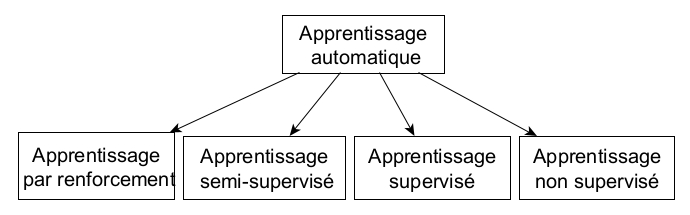
\includegraphics[height=5cm]{ch2-ml-tree-01.jpg}
	\caption{Paradigmes d'apprentissage automatique}
    \label{fig:ch2-ml-tree-01}
\end{figure}

\begin{enumerate}
\item [$\bullet$] \textbf{Apprentissage supervisé} : dans ce type d'apprentissage, les algorithmes sont entraînés sur des données étiquetées. 
Une fois que le modèle est généré, il peut être utilisé pour faire des prédictions sur de nouvelles données en inférant les étiquettes correspondantes en fonction des caractéristiques observées.\\
Les problèmes d'apprentissage supervisé peuvent être catégorisés en deux types principaux : la régression et la classification. Dans la régression, l'objectif est de prédire une valeur numérique continue. Les algorithmes couramment utilisés pour la régression comprennent la régression linéaire, la régression à vecteurs de support, les arbres de régression, les forêts aléatoires, et les réseaux de neurones de régression.
\\
Dans la classification, l'objectif est de prédire une étiquette ou une classe spécifique. Les algorithmes couramment utilisés pour la classification comprennent les arbres de décision, les forêts aléatoires, les machines à vecteurs de support (SVM), les méthodes de régression logistique, les réseaux de neurones et les algorithmes de classification bayésienne \cite{ch_Deep_Learning}.

\item [$\bullet$] \textbf{Apprentissage non supervisé} : cherche à identifier des structures, des modèles (patterns) ou des relations dans les données non étiquetées. Cela peut être réalisé à l'aide de techniques telles que le partitionnement de données (clustering), la réduction de dimensionalité, les règles d'association \cite{ch_Deep_Learning}, etc. 

\item [$\bullet$] \textbf{Apprentissage semi-supervisé } : est une combinaison des deux types d'apprentissage précédents, où le modèle est généré en utilisant à la fois des données étiquetées et non étiquetées. Cette méthode est utile lorsque les données étiquetées sont limitées ou coûteuses à obtenir. Elle vise à exploiter les informations contenues dans les données non étiquetées pour améliorer les performances de généralisation du modèle.
\\
Les algorithmes d'apprentissage semi-supervisé impliquent généralement deux étapes principales : l'entraînement initial sur les données étiquetées et la propagation des étiquettes aux données non étiquetées. L'entraînement initial est effectué à l'aide des exemples étiquetés pour construire un modèle de prédiction. Ensuite, les étiquettes prédites sont exploitées pour prédire les étiquettes des exemples non étiquetés \cite{semi-supervise_chapelle2006semi}.

\item [$\bullet$] \textbf{Apprentissage par renforcement} : est une technique d'apprentissage automatique où un agent apprend à prendre des décisions dans un environnement en interagissant avec celui-ci. L'agent reçoit des récompenses ou des pénalités en fonction de ses actions et apprend à optimiser ses actions pour maximiser les récompenses à long terme. Parmi les algorithmes les plus reconnus de l'apprentissage par renforcement, on peut citer Q learning \cite{q_learning_01} et policy gradient \cite{policy_gradient_01}.
\end{enumerate}
Le choix du modèle d'apprentissage à appliquer dépend de la nature des données disponibles,de la complexité du problème, des ressources disponibles et des objectifs spécifiques de l'application.
\section{Apprentissage profond}
L'apprentissage profond (connu sous le nom de deep learning en anglais) a provoqué une véritable révolution dans le domaine de l'apprentissage automatique. Il a ouvert la voie à la création de modèles de plus en plus complexes et, dans une certaine mesure, plus précis, capables de résoudre des problèmes difficiles dans les domaines de la vision par ordinateur, le traitement du langage naturel, la reconnaissance vocale, et bien d'autres encore \cite{ch_Deep_Learning}.

Ces avancées ont surmonté les limitations des méthodes classiques d'apprentissage en termes de performances. En effet, ces méthodes nécessitent souvent une intervention humaine pour extraire des caractéristiques significatives à partir des données d'entrée, ce qui a limité leur capacité de  généralisation \cite{ch_Deep_Learning}.

Avant l'émergence de l'apprentissage en profondeur, les méthodes d'apprentissage automatique étaient principalement basées sur des algorithmes d'apprentissage supervisé ou non supervisé tels que les arbres de décision, les k-means, les SVM, etc. Ces méthodes étaient limitées par la complexité des modèles qu'elles pouvaient créer et leur capacité à gérer des données complexes et non structurées. Elles nécessitaient souvent une intervention humaine pour extraire des caractéristiques significatives à partir des données d'entrée, ce qui limitait leur capacité à généraliser à de nouvelles données \cite{ch_Deep_Learning}.

L'apprentissage profond repose sur l'utilisation des réseaux de neurones artificiels profonds (DNN), qui permettent une représentation hiérarchique à partir de données brutes sans avoir besoin d'une intervention humaine pour sélectionner des caractéristiques significatives. 
Les DNN sont composés de  multiple couches cachées empilées. Cette architecture en couches contribue à la flexibilité des modèles. Chaque couche apprend à reconnaître des caractéristiques de plus en plus abstraites et complexes. Cela permet au modèle de détecter des relations et de différents patterns dans les données(souvent complexes), ce qui conduit à des prédictions plus précises et à des performances améliorées \cite{ch_Deep_Learning}.

\subsection{Réseaux de neurones artificiels}
Les réseaux de neurones artificiels sont des modèles d'apprentissage statistiques qui imitent le fonctionnement du cerveau humain pour résoudre des problèmes complexes d'apprentissage automatique. Ils sont généralement utilisés pour résoudre des problèmes de classification, de régression et de prédiction \cite{ch_Deep_Learning}.

Un réseau de neurones artificiels est composé des couches de neurones interconnectés. Chaque neurone reçoit des signaux d'entrée pondérés, effectue des calculs sur ces signaux et transmet une sortie à d'autres neurones. Ces connexions entre les neurones sont associées à des poids qui déterminent l'importance de chaque connexion \cite{ch_Deep_Learning}.

L'apprentissage des réseaux de neurones est réalisé par l'ajustement des poids des connexions, de manière à minimiser une fonction d'erreur. Cela se fait généralement à l'aide d'une technique appelée rétropropagation du gradient, qui utilise la dérivée de la fonction d'erreur par rapport aux poids pour mettre à jour les poids du réseau \cite{ch_Deep_Learning}.

Il existe plusieurs types de réseaux de neurones profonds, chacun avec une architecture différente pour résoudre des problèmes spécifiques. Les types de réseaux de neurones artificiels courants incluent :

\begin{outline}
\1  Les réseaux de neurones multi-couches (MLP), également connus sous le nom de réseaux à propagation avant: sont largement largement utilisée en apprentissage automatique. L'architecture de base d'un MLP comprend généralement une couche d'entrée, une ou plusieurs couches cachées et une couche de sortie. Chaque couche est composée de neurones, également appelés perceptrons, qui effectuent des opérations mathématiques sur les entrées pour générer des sorties \cite{MLP_simon2004machine}.

\1  Les réseaux de neurones récurrents (RNN) : sont une classe de réseaux de neurones artificiels conçus pour traiter des données séquentielles ou temporelles. Les RNN ont des connexions récurrentes entre les neurones. Cela signifie que chaque neurone dans un RNN reçoit des entrées non seulement de la couche précédente. Ce qui permet aux RNN de conserver une mémoire à court terme et de traiter des informations passées tout en prenant en compte les informations actuelles \cite{ch_Deep_Learning}.

\1  Les réseaux de neurones convolutifs (CNN) : sont particulièrement adaptée pour le traitement de données structurées en 2D (images) ou 1D (vecteurs). 
Ils utilisent des couches de convolution pour capturer les motifs spatiaux (sur les différents échelles) et les relations locales dans les données \cite{CNN_lecun1998gradient}.

\1  Les réseaux de neurones auto-encodeurs : sont utilisé pour apprendre des représentations compressées des données en utilisant un processus d'encodage et de décodage. L'architecture d'un auto-encodeur comprend généralement trois modules principaux : l'encodeur, la représentation latente et le décodeur. L'encodeur prend les données d'entrée et les transforme en une représentation latente de dimension réduite. Cette représentation latente est ensuite alimentée au décodeur, qui tente de reconstruire les données d'origine à partir de cette représentation latente. L'objectif est de minimiser l'erreur de reconstruction entre les données d'entrée et les données reconstruites. Les auto-encodeurs sont utiles pour la compression, la réduction de dimension, le débruitage des données et la génération de données similaires \cite{auto-encodeurs_hinton2006reducing}.

\end{outline}

\subsection{Réseau de neurones convolutifs}
Selon la figure \ref{fig:CNN}, les réseaux de neurones convolutifs sont constitués des couches suivantes:

\begin{figure}[H]
	\centering
	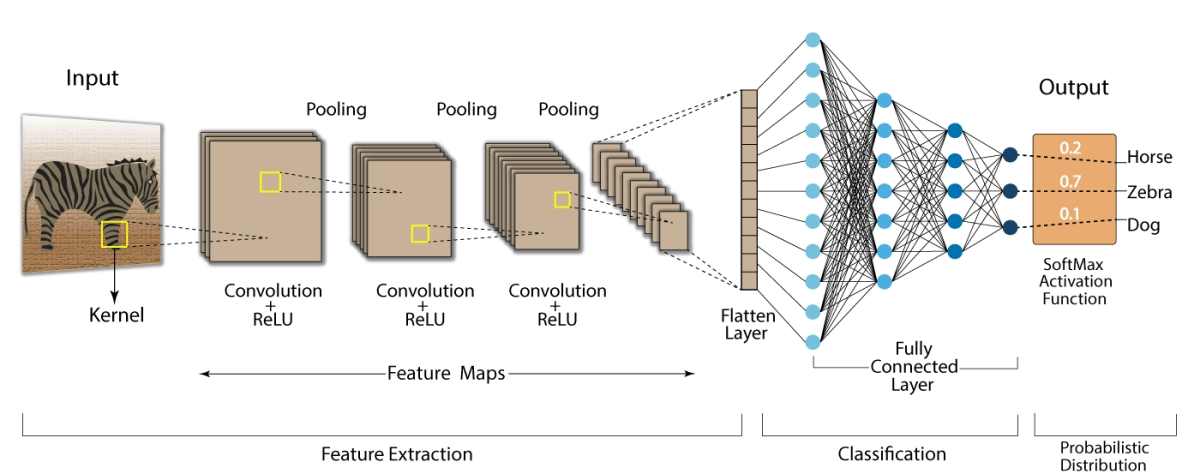
\includegraphics[height=05cm]{ch2-CNN_archi-01.jpg}
	\caption{Réseau de neurones convolutifs}
\label{fig:CNN}
\end{figure}

\textbf{1- Couche de convolution:} cette couche applique des opérations de convolution sur les entrées, à l'aide des filtres, pour extraire des caractéristiques locales et spatiales des données. Chaque filtre est une matrice de poids avec une taille bien définie, qui est appliquée à une fenêtre glissante de l'entrée. Pendant la convolution, les poids du filtre sont multipliés avec les valeurs de la fenêtre d'entrée, puis les produits sont sommés pour obtenir une seule valeur. Ce processus est répété pour chaque position de la fenêtre glissante, couvrant ainsi l'ensemble de l'entrée. Les résultats de ces opérations de convolution sont rassemblés dans une carte d'activation appelée carte des caractéristiques ou feature map.
la figure \ref{fig:convolution} montre l'opération de convolution sur une matrice en entrée \cite{cnn_Agronomy86}.

\begin{figure}[H]
	\centering
	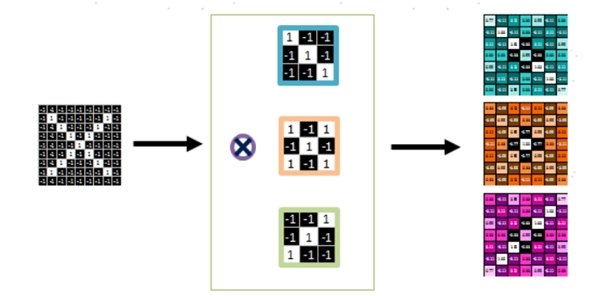
\includegraphics[height=05cm]{ch2-cnn-Couche de convolution.jpg}
	\caption{Convolution d'une image}
 \label{fig:convolution}
\end{figure}

\textbf{2- Couche de mise en commun (pooling) :} selon la figure \ref{fig:pooling}, la couche pooling consiste à diminuer la dimensionnalité des caractéristiques extraites par la couche de convolution d'un CNN. Son objectif est de conserver les informations les plus importantes tout en réduisant le nombre de paramètres et en évitant le sur-apprentissage. L'opération de mise en commun se fait en utilisant une fenêtre (généralement de taille 2x2 pixels) qui se déplace sur les cartes des caractéristiques. À chaque position de la fenêtre, la valeur maximale (ou parfois la moyenne) des pixels couverts par la fenêtre est conservée, tandis que les autres valeurs sont ignorées \cite{makina-corpus}.

\begin{figure}[H]
	\centering
	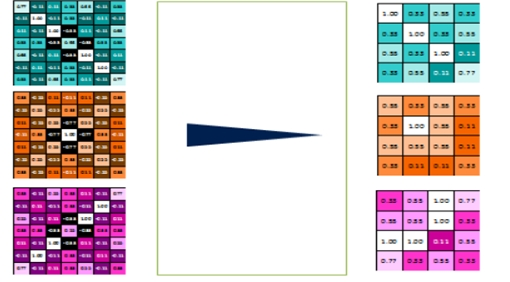
\includegraphics[height=05cm]{ch2-cnn-pooling.jpg}
	\caption{Opération de mise en commun}
 \label{fig:pooling}
\end{figure}

\textbf{3- couche entièrement connectée(dense ou fully connected en anglais):}
joue un rôle fondamental au sein des CNN. Chaque neurone au sein de cette couche est connecté à tous les neurones de la couche précédente, avec des poids définis pour chaque connexion. Les entrées sont soumises à un processus de pondération et de sommation, suivi de l'application d'une fonction d'activation non linéaire telle que la sigmoïde, la ReLU (Rectified Linear Activation), la tangente hyperbolique (tanh), et autres. Cette fonction d'activation permet au réseau de saisir les relations complexes entre les données en introduisant des seuils et des non-linéarités dans les calculs. Les couches entièrement connectées sont fréquemment positionnées vers la fin d'un réseau de neurones afin de fusionner et combiner les caractéristiques apprises des couches précédentes, en vue de produire en fin de compte une sortie finale correspondant aux prédictions du modèle, telles que la classification d'une image ou la prédiction d'une valeur numérique, par exemple \cite{makina-corpus}..Et c'est ce qui est représenté sur la figure \ref{fig:fully},
\begin{figure}[H]
	\centering
	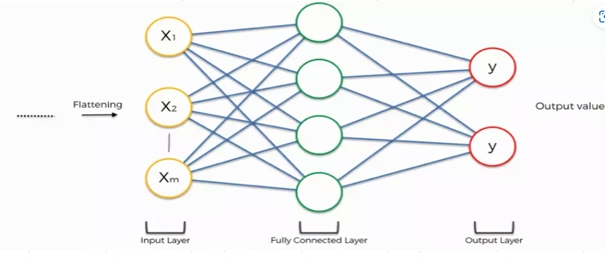
\includegraphics[height=05cm]{ch2-cnn-full connection.jpg}
	\caption{Couche entièrement connectée}
 \label{fig:fully}
\end{figure}

%-- https://datascientest.com/convolutional-neural-network
%   https://makina-corpus.com/sig-webmapping/extraction-dobjets-pour-la-cartographie-par-deep-learning-choix-du-modele

\subsection{Architectures CNN}
Un éventail d'architectures majeures a été développé, parmi lesquelles nous pouvons mentionner :
\begin{outline}
\1 LeNet: développé par Yann LeCun en 1998, a été l'un des premiers réseaux de neurones convolutifs à gagner en popularité. Il a été spécifiquement conçu pour la reconnaissance de chiffres manuscrits. Cette architecture comportait plusieurs couches de convolution et de sous-échantillonnage, ainsi que des couches entièrement connectées à la fin. Bien que relativement simple par rapport aux architectures modernes, LeNet a ouvert la voie à la compréhension de la puissance des CNN dans la vision par ordinateur \cite{vitalflux2023different}.

\1 AlexNet: présenté en 2012 par Alex Krizhevsky et son équipe, a marqué un tournant dans l'utilisation des CNN pour la classification d'images. Il a remporté le concours ImageNet en 2012 en obtenant une précision remarquable. AlexNet a introduit l'utilisation répandue de la fonction d'activation ReLU et a montré comment l'augmentation des données d'entraînement pouvait grandement améliorer les performances du modèle. Cette architecture comportait des couches de convolution, de pooling et des couches entièrement connectées, créant un précédent pour les CNN modernes \cite{vitalflux2023different}.

\1 VGGNet : proposé en 2014 par Simonyan et Zisserman, a été remarquable pour sa profondeur. Cette architecture avait une structure très uniforme avec plusieurs couches de convolution de taille 3x3, suivies de couches de pooling, et enfin de couches entièrement connectées. Bien que VGGNet soit plus profond que les modèles précédents, sa simplicité a permis de mieux comprendre comment la profondeur du réseau peut influencer la performance \cite{analyticsvidhya2019vggnet}.

\1 GoogLeNet (Inception) : également connu sous le nom d'Inception, est une architecture révolutionnaire introduite par Szegedy et son équipe en 2014. Elle a introduit le concept de modules Inception, où plusieurs filtres de différentes tailles sont appliqués en parallèle pour capturer des caractéristiques à différentes échelles. Cela a permis d'obtenir des performances de pointe tout en maintenant une complexité relativement faible, grâce à l'utilisation efficace des opérations de convolution \cite{medium-article}.

\1 ResNet (Residual Network) : L'architecture ResNet, présentée en 2015 par Kaiming He et ses collaborateurs, a abordé le problème du "vanishing gradient" en introduisant les blocs résiduels. Ces blocs utilisaient des connexions de saut (skip connections) pour ajouter directement les sorties des couches précédentes aux couches suivantes. Cela a permis la formation de réseaux extrêmement profonds sans subir de dégradation de performance due au problème du gradient. Les ResNets ont ouvert la voie à la création de modèles encore plus profonds et performants \cite{geeksforgeeks-resnet}.
\end{outline}

Chacune de ces architectures a contribué de manière significative à l'avancement des CNN en introduisant des idées novatrices pour la capture de caractéristiques et la gestion de la profondeur. Elles occupent une place essentielle dans le domaine de la vision par ordinateur en permettant l'extraction automatique de caractéristiques visuelles à partir de données complexes, particulièrement dans des domaines tels que la détection d'objets.

Le tableau \ref{tab:my-table} illustre une série de modèles CNN qui sont intégrés automatiquement dans le framework Keras, ainsi que les caractéristiques respectives: taille (en MB), exactitude top-1, exactitude top-5, nombre de paramètres, profondeur du modèle et temps d'exécutionen en ms (CPU/ GPU) \cite{ch2_KerasApp87}.

\begin{table}[h]
\centering
\caption{Modèles CNN prédéfinis dans le framework Keras \cite{ch2_KerasApp87}.}
\label{tab:my-table}
\resizebox{\columnwidth}{!}
{
    \begin{tabular}{|l|l|l|l|l|l|p{2cm}|p{2cm}|}
    \hline
    Modèle & Taille & Exactitude top-1 & Exactitude top-5  & Paramètres & Profondeur & Temps (CPU)(MS) & Temps (GPU)(MS) \\
    \hline
    Xception          & 88     & 79.00\% & 94.50\% & 22.9M  & 81  & 109.4  & 8.1  \\
    VGG16             & 528    & 71.30\% & 90.10\% & 138.4M & 16  & 69.5   & 4.2  \\
    VGG19             & 549    & 71.30\% & 90.00\% & 143.7M & 19  & 84.8   & 4.4  \\
    ResNet50          & 98     & 74.90\% & 92.10\% & 25.6M  & 107 & 58.2   & 4.6  \\
    ResNet50V2        & 98     & 76.00\% & 93.00\% & 25.6M  & 103 & 45.6   & 4.4  \\
    ResNet101         & 171    & 76.40\% & 92.80\% & 44.7M  & 209 & 89.6   & 5.2  \\
    ResNet101V2       & 171    & 77.20\% & 93.80\% & 44.7M  & 205 & 72.7   & 5.4  \\
    ResNet152         & 232    & 76.60\% & 93.10\% & 60.4M  & 311 & 127.4  & 6.5  \\
    ResNet152V2       & 232    & 78.00\% & 94.20\% & 60.4M  & 307 & 107.5  & 6.6  \\
    EfficientNetB0    & 29     & 77.10\% & 93.30\% & 5.3M   & 132 & 46     & 4.9  \\
    \hline  
    \end{tabular}   
}
\end{table}

\subsection{Apprentissage par transfert}

L'apprentissage par transfert est une approche dans le domaine de l'apprentissage automatique où les connaissances et les modèles acquis lors de la résolution d'une tâche sont transférés pour aider à résoudre une tâche similaire ou connexe. Plutôt que de construire un modèle à partir de zéro pour chaque nouvelle tâche, on utilise les informations déjà apprises dans le cadre d'une tâche précédente pour accélérer et améliorer l'apprentissage d'une nouvelle tâche \cite{Transfer_Transfer32}.\\
Les avantages de l'apprentissage par transfert sont nombreux, notamment la réduction du temps et des ressources nécessaires pour entraîner un modèle, une meilleure généralisation sur de petits ensembles de données, et la possibilité d'appliquer des connaissances d'un domaine à un autre \cite{Transfer_WhatIsTr80}.\\
Cependant, le succès de l'apprentissage par transfert dépend de la similitude entre les tâches sources et cibles. Si les tâches sont trop différentes, le transfert peut ne pas être aussi efficace. Les techniques d'apprentissage par transfert incluent le transfert de caractéristiques (où les couches basses d'un modèle préalablement formé sont utilisées comme extracteurs de caractéristiques), le transfert de connaissances (où des connaissances spécifiques à une tâche sont transférées), et l'adaptation fine (où un modèle préalablement formé est ajusté pour mieux s'adapter à une tâche spécifique) \cite{Transfer_Transfer45}.

\section{ Vision par ordinateur}

La vision par ordinateur constitue un champ interdisciplinaire qui fait partie de l'intelligence artificielle. Il se concentre sur la conception d'ordinateurs capables d'acquérir une compréhension avancée à partir de données visuelles, telles que des images ou des vidéos numériques. D'un point de vue d'ingénierie, son objectif est d'automatiser les fonctions réalisables par le système visuel humain \cite{Vision_par_ordinateur_Computer61}. 

\begin{figure}[H]
	\centering
	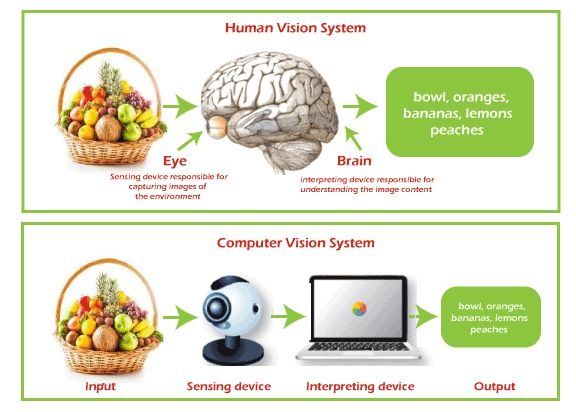
\includegraphics[height=07cm]{ch2-process_cv.jpg}
	\caption{Processus de la vision par ordinateur}
    \label{ch2-process_cv}
\end{figure}

Son évolution, grâce à l'apprentissage automatique et profond, a été marquée par des progrès significatifs. Depuis les années 1960, avec les premiers programmes de reconnaissance de caractères imprimés, la vision par ordinateur est passée d'algorithmes basés sur des règles à des méthodes traitant des tâches complexes. L'arrivée de l'apprentissage automatique dans les années 1990 a ouvert de nouvelles perspectives, permettant aux ordinateurs d'apprendre à partir de données plutôt que de règles prédéfinies. Ceci a amélioré leur performance dans différents problèmes notamment dans la détection d'objets. La figure \ref{ch2-process_cv} présente la relation entre l'intelligence artificielle et ses divers domaines en lien avec la vision par ordinateur.

\subsection{Techniques de la vision par ordinateur}
Les techniques de la vision par ordinateur sont des méthodes et des approches utilisées pour traiter et analyser des données visuelles, notamment des images et des vidéos \cite{javatpoint2023computer}. Certaines des techniques les plus importantes et couramment utilisées dans ce domaine comprennent Et montré sur la figure \ref{fig:ch2-Techniques_cv}:

\begin{itemize}
    \item  \textbf{Classification d'images} : Prédire la classe d'une image en fonction de son contenu visuel.
    \item  \textbf{Détection d'objets} : Localiser et identifier la présence d'objets spécifiques dans une image.
    \item  \textbf{Détection des points d'intérêt} : Identifier et localiser de caractéristiques significatives (points, coins, blobs, ... etc.) dans une image.
    \item  \textbf{Segmentation d'objets (ou sémantique)} : Diviser une image en régions pour identifier les parties spécifiques des objets.
    \item  \textbf{Reconnaissance de formes} : Identifier des motifs spécifiques dans les données visuelles.
    \item  \textbf{Suivi d'objets} : Suivre les mouvements et les interactions des objets dans une séquence d'images.
    \item  \textbf{Segmentation d'instances} : Identifier et séparer chaque instance d'objet distincte au sein d'une image.
    \item  \textbf{Reconstruction 3D} : Créer des modèles tridimensionnels à partir d'images bidimensionnelles.
    \item  \textbf{Estimation de mouvement} : Déterminer les mouvements et les déplacements des objets dans une séquence d'images.

Ces techniques sont largement utilisées pour résoudre une variété de problèmes de vision par ordinateur, allant de l'analyse d'images médicales à la navigation autonome des véhicules.
\end{itemize}

\begin{figure}[H]
	\centering
	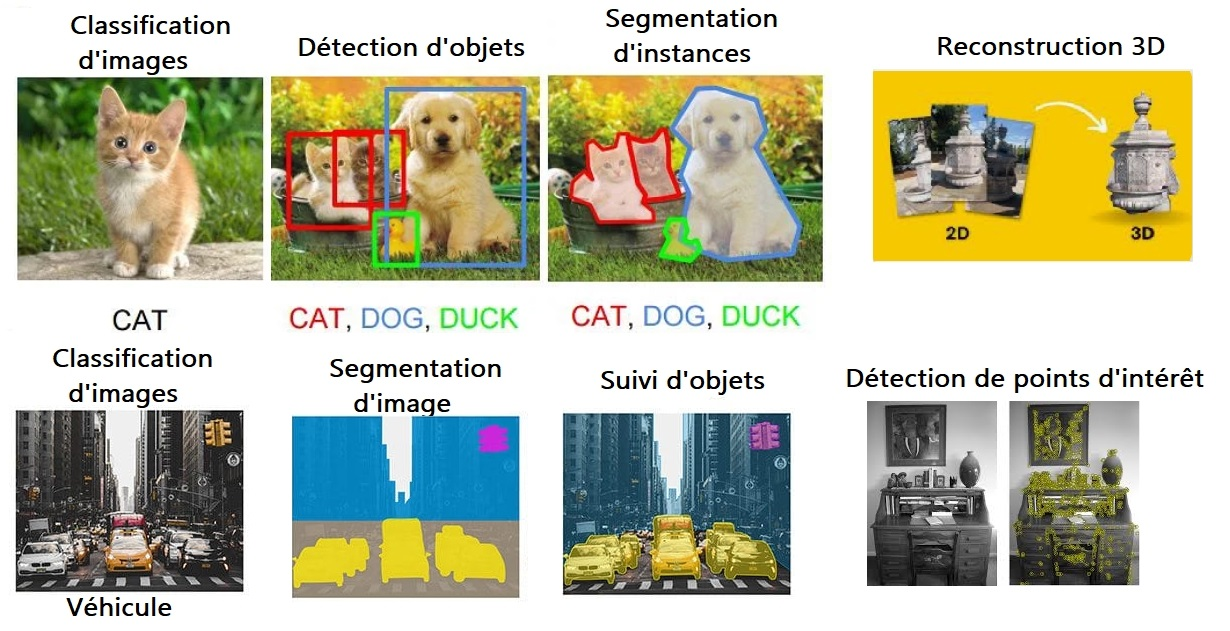
\includegraphics[height=08cm]{ch2-Techniques_cv.jpg}
	\caption{Techniques de la vision par ordinateur \cite{simplilearn2023computer}}
    \label{fig:ch2-Techniques_cv}
\end{figure}

\subsection{Applications de la vision par ordinateur }

La vision par ordinateur est utilisée dans des domaines variés \cite{simplilearn2023computer}, notamment:

\subsubsection{ Véhicules autonomes }
Grâce à des caméras et des algorithmes de vision, les véhicules autonomes peuvent percevoir leur environnement, détecter les bords de la route, les panneaux de signalisation, autres véhicules, obstacles et piétons, leur permettant de naviguer en toute sécurité \cite{simplilearn2023computer}.

\subsubsection{Reconnaissance faciale }
Les algorithmes de reconnaissance faciale utilisent la vision par ordinateur pour identifier des individus dans des images. Ils identifient les caractéristiques du visage, les comparant à des profils enregistrés. Cela a des applications allant de la vérification d'identité sur les appareils électroniques grand public à l'application dans les réseaux sociaux et les forces de l'ordre \cite{simplilearn2023computer}.

\subsubsection{Réalité augmentée et mixte }
La vision par ordinateur est essentielle pour la réalité augmentée, où des éléments numériques sont superposés sur le monde réel via des caméras. Ces technologies utilisent la vision par ordinateur pour reconnaître les surfaces et positionner correctement les éléments virtuels dans l'environnement réel \cite{simplilearn2023computer}.

\subsubsection{Santé }
La vision par ordinateur a transformé le secteur médical en automatisant des tâches telles que la détection de problèmes dermatologiques ou l'analyse d'images médicales comme les radiographies et les IRM, ce qui accélère les diagnostics et les traitements \cite{simplilearn2023computer}.

\section{Algorithmes de détection d'objets}

La détection d'objets au sein d'images ou de séquences d'images constitue une application cruciale de la vision par ordinateur. Cette technologie trouve des applications variées, telles que la surveillance, l'automatisation industrielle, la robotique, la sécurité et les véhicules autonomes, entre autres. Pour accomplir cette tâche complexe, une gamme d'algorithmes est utilisée. Ces méthodes peuvent être regroupées en deux catégories principales : les détecteurs à un seul niveau et les détecteurs à deux niveaux, en fonction du schéma illustré dans la figure \ref{ch2-oneStage-twoStage-01}.

\begin{figure}[H]
	\centering
	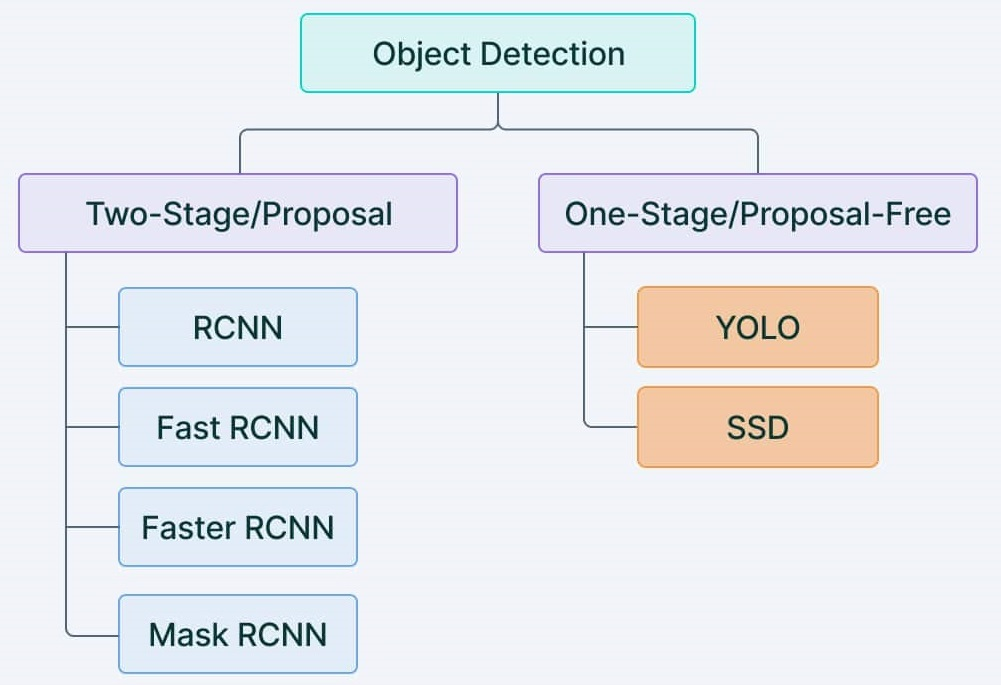
\includegraphics[height=08cm]{ch2-oneStage-twoStage-01.jpg}
	\caption{Classification des algorithmes de détection d'objets }
 \label{ch2-oneStage-twoStage-01}
\end{figure}

\subsubsection{Détecteurs d'objets à deux niveaux}
La  détection d'objets à deux niveaux (two-shot object detection ) fait référence à une approche en deux étapes pour détecter et localiser des objets au sein d'une image \cite{ch2_The5Comp69}.
Dans un détecteur d'objets à deux niveaux, la détection se fait en deux étapes distinctes :
\begin{itemize}
    \item [(1)] Génération de propositions (régions d'intérêt) : Dans la première étape, le modèle génère des régions d'intérêt qui pourraient potentiellement contenir des objets. Ces régions sont extraites en utilisant des techniques telles que les régions de haute probabilité basées sur des caractéristiques visuelles. Cela réduit le nombre de régions à examiner plus en détail dans la prochaine étape.
    \item [(2)] Classification et localisation : Dans la deuxième étape, les régions d'intérêt générées sont soumises à des modèles de classification et de localisation. Le modèle classe chaque région comme contenant un certain type d'objet ou non, et ajuste également les boîtes englobantes autour de ces objets.
\end{itemize}

Cette approche offre plus de précision mais potentiellement plus lente.

\subsubsection{Détecteurs d'objets à un niveau}  
Dans la détection d'objets à un niveau (single-shot object detection), la détection et la classification des objets sont effectuées simultanément en une seule étape, sans nécessiter une étape distincte de génération de propositions \cite{ch2_The5Comp69}.

Dans les détecteurs d'objets à un seul niveau, l'algorithme prédit directement les boîtes englobantes des objets ainsi que leurs étiquettes de classe correspondantes. Cela simplifie le processus en éliminant le besoin de générer d'abord des propositions de région, puis de les classifier et de les affiner comme dans les détecteurs à deux niveaux. \\
Bien que les détecteurs à un seul niveau offrent des avantages en termes de vitesse, ils peuvent parfois sacrifier une certaine précision par rapport aux détecteurs à deux niveaux en raison de la nature directe et simultanée de leurs prédictions \cite{ch2_The5Comp69}.\\

\subsection{RCNN}
RCNN (Region-based Convolutional Neural Network) a été l'une des premières approches populaires pour la détection d'objets basée sur CNN. Il fonctionne selon les étapes suivantes: 
\begin{itemize}
    \item Proposition de régions : La première étape de RCNN consiste à générer un ensemble de régions d'intérêt (ROIs) dans une image. Cela se fait généralement à l'aide d'une méthode de propositions de régions, telle que selective search. Cette dernière parcourt l'image pour identifier des régions qui semblent contenir des objets et les propose comme ROIs. Ces ROIs peuvent être de différentes tailles et formes \cite{ch2_The5Comp69}.
    \item Extraction de caractéristiques : Une fois que les ROIs ont été identifiées, chaque ROI est découpée de l'image originale et redimensionnée pour avoir une taille fixe. Ensuite, un CNN pré-entraîné, comme VGG16 ou autre, est utilisé pour extraire des caractéristiques de chaque ROI. Le CNN transforme l'image de la ROI en un vecteur de caractéristiques de dimension fixe \cite{ch2_The5Comp69}.
    \item Classification : Les vecteurs de caractéristiques extraits de chaque ROI sont ensuite introduits dans un classifier. Ce dernier est généralement une couche entièrement connectée qui attribue une classe (parmi les classes d'objets prédéfinies) à chaque ROI. Il s'agit de déterminer quelle est la nature de l'objet contenu dans la ROI \cite{ch2_The5Comp69}.
    \item Régression des boîtes de délimitation : En plus de la classification, RCNN effectue également une régression des boîtes de délimitation autour des objets. Cela signifie qu'il ajuste les coordonnées des boîtes englobantes autour des objets pour les rendre plus précises \cite{ch2_The5Comp69}.
    \item Non-maximum suppression : Après avoir effectué la classification et la régression, RCNN applique une méthode connue sous le nom de suppression des non-maxima (NMS) pour éliminer les détections redondantes ou peu fiables, assurant ainsi que chaque objet n'est détecté qu'une seule fois. Cette technique repose sur la mesure "IoU" (Intersection Over Union) \cite{ch2_The5Comp69}.
\end{itemize}
Cependant, une limitation majeure de RCNN est sa lenteur en raison du traitement indépendant des ROIs, ce qui a conduit au développement de versions plus rapides et efficaces telles que Fast R-CNN et Faster R-CNN.


\subsection{Fast R-CNN} 
Fast R-CNN est une amélioration significative par rapport à RCNN en termes d'efficacité \cite{ren2015fasterarxiv}. Il élimine la nécessité de traiter chaque ROI indépendamment. Au lieu de cela, il utilise une seule passe CNN sur l'image entière pour extraire des caractéristiques. Les ROIs sont ensuite alignées avec les caractéristiques extraites de l'image globale.
Fast R-CNN a été plus rapide que RCNN car il évite de répéter le calcul coûteux des caractéristiques pour chaque ROI.
Fast R-CNN se distingue par sa rapidité par rapport à RCNN, car il élimine la nécessité de recalculer les caractéristiques  pour chaque ROI \cite{ch2_The5Comp69}.


\subsection{Faster R-CNN}
Faster R-CNN est une autre amélioration majeure par rapport à Fast R-CNN. Selon la figure \ref{FasterRCNN}, Faster R-CNN (Faster Region-based Convolutional Neural Network) \cite{ren2015faster} se compose de plusieurs composants clés qui travaillent ensemble pour effectuer la détection d'objets :
\begin{itemize}
    \item CNN: l'architecture commence par un réseau neuronal convolutif de base, tel que VGG16 ou des modèles similaires. Ce réseau extrait des caractéristiques de l'image d'entrée, créant ainsi une carte de caractéristiques qui encode des informations visuelles importantes \cite{ch2_The5Comp69}.
    \item Réseau de proposition de régions (RPN) : est intégré au réseau neuronal de base et génère directement des propositions de régions à partir de la carte de caractéristiques. Ces propositions sont des régions potentielles où des objets pourraient être présents. Le RPN suggère des régions en fonction de boîtes d'ancrage (boîtes prédéfinies de différentes tailles et rapports d'aspect) et prédit la probabilité de présence d'un objet ainsi que les ajustements à apporter aux boîtes d'ancrage pour bien encadrer les objets \cite{ch2_The5Comp69}.
    \item RoI pooling (ou RoI Align) : les régions proposées par le RPN sont alignées sur une taille et une forme fixes (par exemple, 7x7) à l'aide de RoI pooling ou RoI align. Cette étape garantit que les caractéristiques des régions ont une taille cohérente, ce qui est nécessaire pour les tâches de classification et de régression qui suivent \cite{ch2_The5Comp69}.
    \item Tête de détection (classification et régression des boîtes englobantes): les caractéristiques des régions alignées sont introduites dans une tête de classification, qui prédit la probabilité que chaque région proposée contienne différentes classes d'objets. Cette classification est généralement effectuée à l'aide de couches entièrement connectées ou de convolutions 1x1.
    De plus, les mêmes caractéristiques passent par la tête de régression des boîtes englobantes, qui ajuste les paramètres des boîtes d'ancrage pour obtenir une adaptation précise des boîtes englobantes des objets détectés \cite{ch2_The5Comp69}.  
\end{itemize}

\begin{figure}[H]
	\centering
	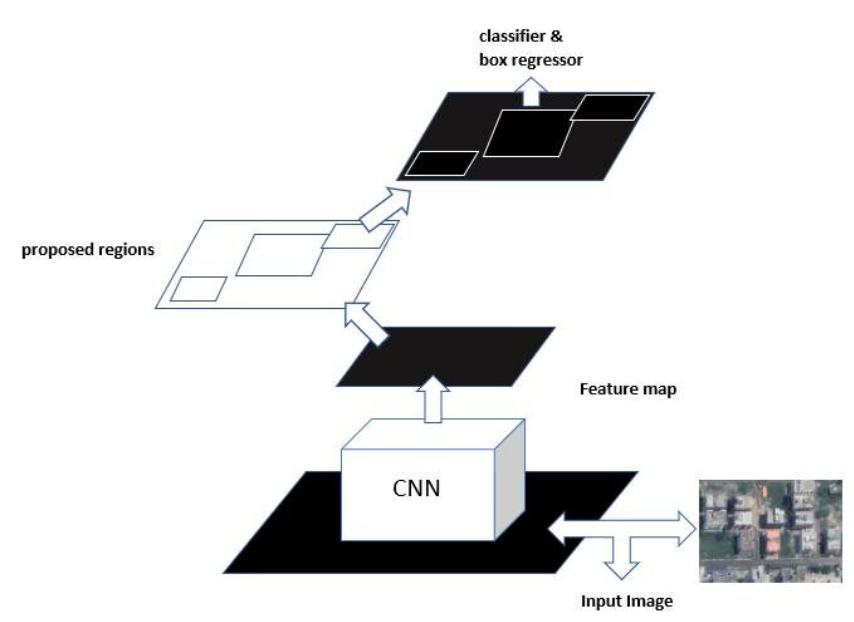
\includegraphics[height=07cm]{img/Faster-R-CNN2.png}
	\caption{L'architecture du Faster R-CNN}
 \label{FasterRCNN}
\end{figure}

\subsection{SSD}
Le SSD (Single Shot MutiBox Detector) est un détecteur capable de détecter plusieurs objets à différentes échelles en une seule étape, comme illustré dans la figure \ref{SSD}. Il réalise cette détection en prédisant des boîtes d'ancrage de différentes tailles et proportions \cite{liu2016ssd}. L'architecture SSD  est composée de plusieurs composants, notamment :
\begin{itemize}
    \item Backbone convolutif : SSD utilise un réseau de neurones convolutifs profonds pré-entraîné, généralement basé sur des architectures telles que VGG16 , comme base pour extraire des caractéristiques d'image. Ce réseau sert de "backbone" pour le modèle \cite{ch2_The5Comp69}.
    \item Pyramide de caractéristiques (feature pyramid) : SSD construit une pyramide de caractéristiques en ajoutant des couches de convolution supplémentaires au réseau de base. Ces couches sont conçues pour capturer des informations à différentes échelles spatiales, ce qui permet de détecter des objets de différentes tailles \cite{ch2_The5Comp69}.
    \item Boîtes d'ancrage (anchor boxes) : Pour chaque cellule de la pyramide de caractéristiques, SSD prédit un ensemble de boîtes d'ancrage de différentes tailles et rapports (aspect ratios). Ces boîtes d'ancrage servent de points de référence pour la détection d'objets \cite{ch2_The5Comp69}.
    \item Prédiction des boîtes multibox : Pour chaque boîte d'ancrage, SSD prédit à la fois les décalages (offsets) par rapport à la boîte d'ancrage et les scores de classification pour chaque classe d'objet. Cela signifie qu'il prédit à la fois où se trouve l'objet par rapport à la boîte d'ancrage et quelle est la classe de l'objet.
    Après la prédiction des boîtes MultiBox, SSD applique une étape de non-maximum suppression pour éliminer les détections redondantes et ne conserver que les détections les plus fiables \cite{ch2_The5Comp69}.
\end{itemize}

 
Pour l'apprentissage du modèle SSD, il utilise une fonction de perte qui prend en compte à la fois la classification (score de confiance) et la régression (décalage par rapport aux boîtes d'ancrage) pour entraîner le modèle. Cela inclut généralement une perte de classification et une perte de régression.
   
L'architecture SSD est très efficace pour la détection d'objets en temps réel. 

\begin{figure}[H]
	\centering
	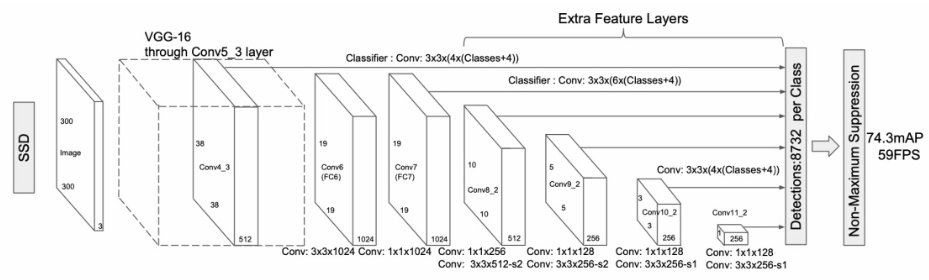
\includegraphics[height=5cm]{ch2-SSD.png}
	\caption{L'architecture du détecteur SSD}
    \label{SSD}
\end{figure}


\subsection{YOLO}
L'algorithme YOLO (You Only Look Once) représente une avancée révolutionnaire en matière de détection d'objets, car il analyse l'intégralité d'une image en une seule itération au travers un CNN \cite{redmon2016yolo}. Son architecture se décompose comme suit :
\begin{itemize}
    \item Couche d'entrée : L'image d'entrée est divisée en une grille de cellules. Chaque cellule est responsable de la détection des objets dans sa région.
    \item  Réseau "backbone": YOLO utilise un CNN pour extraire des caractéristiques importantes de l'image. Il prend en compte l'ensemble de la grille et capture des informations à différentes échelles spatiales.
    \item "Neck": est habituellement constitué de couches de convolution supplémentaires visant à 
    agréger les caractéristiques extraites de la grille à différentes résolutions spatiales et effectue des opérations de fusion pour intégrer des informations provenant de différentes échelles.
    \item Tête de prédiction: comprend des couches de convolution spécifiques pour produire les prédictions. Pour chaque grille, YOLO prédit un certain nombre de boîtes englobantes et les probabilités associées à différentes classes d'objets. Chaque boîte englobante est caractérisée par ses coordonnées (coordonnées x et y de son centre, largeur et hauteur) et les probabilités de classe correspondantes.
    
    Après les prédictions, YOLO applique une étape de non-maximum suppression pour éliminer les boîtes englobantes redondantes et ne conserver que les détections les plus fiables.
\end{itemize}

L'architecture du modèle \cite{ch2_YOLOdéte70} se compose de 24 couches convolutives pour extraire les cartes de caractéristiques suivies de 2 couches entièrement connectées pour réaliser la détection d'objets, comme illustré dans la figure \ref{YOLOarc}.
\begin{figure}[H]
	\centering
	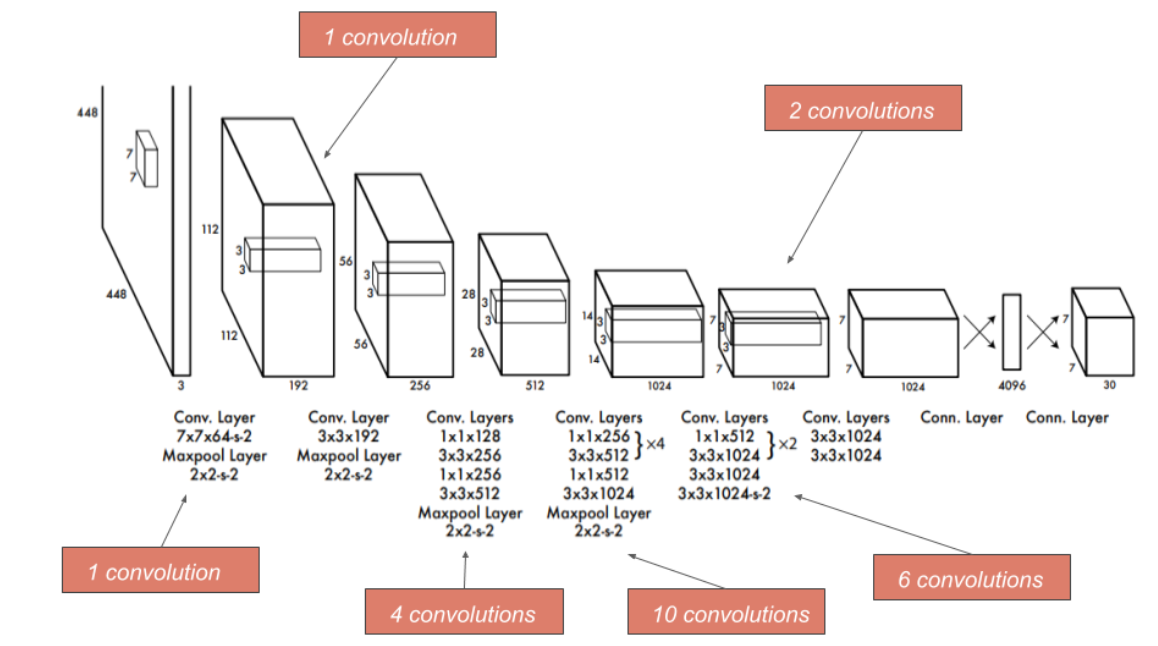
\includegraphics[height=8cm]{ch2-yolo_arch.png}
	\caption{L'architecture du détecteur YOLO}
 \label{YOLOarc}
\end{figure}

YOLO est connu pour sa rapidité et sa précision, car il évite la nécessité de générer des propositions de régions ou de passer plusieurs fois à travers le réseau. Il est couramment utilisé dans des applications telles que la détection d'objets en temps réel, la surveillance vidéo, la conduite autonome et bien d'autres.
\\
Plusieurs versions de YOLO \cite{AGuideto8}ont été développées pour améliorer les performances de la détection, notamment:
YOLOv1 (Juin, 2015),
YOLOv2 (Dec, 2016),
YOLOv3 (Avr, 2018),
YOLOv4 (Avr, 2020),
YOLOv5 (Mai, 2020),
YOLOv6,
YOLOv7,
YOLOv8.

\begin{figure}[H]
	\centering
	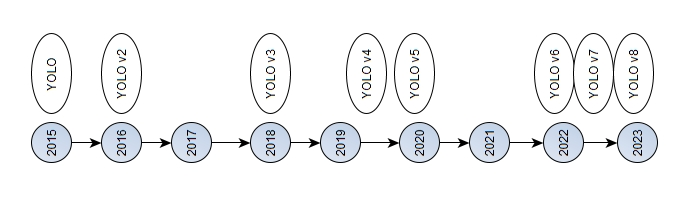
\includegraphics[height=05cm]{ch2-cnn-yolo-all.jpg}
	\caption{Les versions de l'algorithme YOLO}
 \label{YOLO}
\end{figure}

Les principales améliorations de YOLOv8 \footnote{\url{https://blog.roboflow.com/whats-new-in-yolov8/}} incluent l'introduction d'un nouveau réseau fédérateur, une tête divisée innovante sans ancrage, ainsi que de nouvelles fonctions de perte. Ces améliorations permettent à YOLOv8 d'obtenir des performances exceptionnelles tout en conservant une empreinte mémoire réduite et une vitesse d'entraînement remarquable.\\
D'après l'architecture illustrée dans la figure \ref{fig:ch2-yolov8_arch}, ce réseau requiert une image d'entrée de forme carrée, avec une longueur de côté qui doit être un multiple de 32. La forme de l'entrée est couramment représentée comme (3, imgsz, imgsz), où :

\begin{outline}
    \1 "3" indique qu'il y a trois canaux de couleur (rouge, vert, bleu) dans l'image.
    \1 "imgsz" représente la largeur (w) et la hauteur(h) de l'image, qui sont identiques (h=w).
\end{outline}
La sortie du réseau YOLOv8 est représentée sous la forme d'une matrice avec une largeur et une hauteur.
\begin{equation}
\textbf{Largeur} = \text{nombre de classes} + 4
\end{equation}
La hauteur de cette matrice dépend de la taille de l'image d'entrée et est calculée de la manière suivante:
\begin{equation}
\textbf{Hauteur} = 
\left(\frac{{\text{imgsz}}}{{32}}\right)^2 + \left(\frac{{\text{imgsz}}}{{16}}\right)^2 + \left(\frac{{\text{imgsz}}}{{8}}\right)^2
\end{equation}
Chaque ligne de cette matrice représente un objet et est structurée comme suit : [x\_centre de l'objet, y\_centre de l'objet, hauteur, largeur, Score prédiction de classe 1, Score prédiction de classe 2, ...,Score prédiction de classe  N].

\begin{figure}[H]
	\centering
	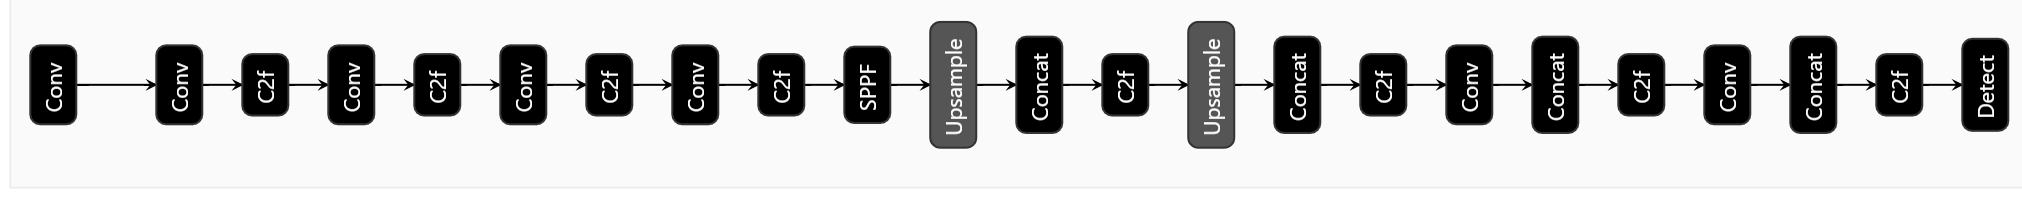
\includegraphics[width=17cm]{ch2-yolov8_arch.png}
	\caption{Architecture du YOLOv8}
    \label{fig:ch2-yolov8_arch}
\end{figure}
% https://github.com/lutzroeder/netron/
% Un programme a été utilisé pour créer ce graphique en utilisant le fichier de poids généré par  yolov8 poid

Il existe cinq extensions du modèle YOLOv8 : YOLOv8n (nano), YOLOv8s (small),YOLOv8m (medium), YOLOv8l (large), YOLOX (eXtra large). YOLOv8 Nano est le plus rapide et le plus petit, tandis que YOLOv8 Extra Large (YOLOv8x) est le plus précis mais aussi le plus lent parmi eux.



\section{Reconnaissance optique de caractères}

L'OCR, ou Optical Character Recognition en anglais (Reconnaissance Optique de Caractères en français), est une technologie qui permet de convertir du texte manuscrit ou imprimé, que ce soit sur du papier ou une image, en texte éditable sur un ordinateur. Cette conversion est réalisée grâce à des ordinateurs et des logiciels spécialement conçus pour analyser les images, extraire les caractères, chiffres et mots, puis les transformer en texte que l'on peut modifier et manipuler \cite{ch2_ocr_definitionxcs}.

Pour illustrer cela, la figure \ref{fig:ch2-ocr_info} montre une image contenant deux mots. Grâce à l'OCR, cette image a été traitée pour produire un texte que l'on peut éditer.

\begin{figure}[H]
	\centering
	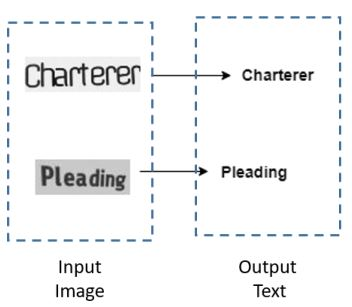
\includegraphics[height=5cm]{ch2-ocr_info.JPG}
	\caption{Reconnaissance optique de caractères}
    \label{fig:ch2-ocr_info}
\end{figure}
En général, le processus d'OCR comprend les étapes suivantes:
\begin{itemize}
    \item [-] Acquisition de l'image : Tout d'abord, une image contenant du texte est acquise à l'aide d'un scanner, d'un appareil photo numérique ou d'un autre moyen de capture d'images. L'image peut contenir du texte imprimé, manuscrit, ou une combinaison des deux.
    \item [-] Prétraitement : L'image capturée peut contenir diverses imperfections telles que des taches, des plis de papier, ou un mauvais contraste. Avant d'effectuer la reconnaissance optique de caractères, l'image est soumise à un prétraitement pour améliorer sa qualité. Cela peut inclure le redressement de l'image, la correction de la luminosité et du contraste, et la suppression du bruit.
    \item [-] Segmentation des caractères : Dans cette étape, l'image est analysée pour séparer les caractères individuels, les mots et les lignes de texte. Cela permet de délimiter clairement chaque élément textuel, ce qui facilite leur traitement ultérieur.
    \item [-] Reconnaissance des caractères : La partie centrale de l'OCR consiste à identifier les caractères individuels présents dans l'image. Cela se fait en comparant les formes des caractères extraits de l'image avec un ensemble de caractères connus. Les algorithmes d'apprentissage automatique, tels que les réseaux neuronaux, sont couramment utilisés pour cette tâche.
    \item [-] Post-traitement : Une fois que les caractères ont été reconnus, des techniques de post-traitement sont souvent appliquées pour corriger les erreurs de reconnaissance éventuelles. Cela peut inclure la vérification de la cohérence du texte, la correction des fautes de frappe, et la reconstruction de mots complets à partir de caractères individuels.
    \item [-] Conversion en texte éditable : Une fois que tous les caractères ont été correctement reconnus et traités, le résultat est converti en texte éditable qui peut être affiché, modifié et sauvegardé sous forme de document texte.
\end{itemize}

\section{Métriques d'évaluation}

Les métriques d'évaluation servent à évaluer la performance et l'efficacité des modèles d'apprentissage et de détection dans des contextes spécifiques. Voici un aperçu des métriques couramment employées pour évaluer ces types de modèles. 
En ce qui concerne l'apprentissage automatique, les mesures suivantes peuvent être calculées \cite{moov-ai-blog} :

\begin{outline}
\1 La matrice de confusion: est un  tableau qui montre le nombre de vrais positifs, de faux positifs, de vrais négatifs  et de faux négatifs. Elle permet une analyse détaillée des performances du modèle.

% --------------------------------------------------------------
\begin{table}[h]
\centering
\begin{tabular}{|c|c|c|}
\hline
                 &  Réels Positifs    & Réels Négatifs     \\
\hline
Prédits Positifs & Vrais Positifs (VP) & Faux Positifs (FP) \\
\hline
Prédits Négatifs & Faux Négatifs (FN) & Vrais Négatifs (VN) \\
\hline
\end{tabular}
\caption{Matrice de Confusion}
\end{table}
% --------------------------------------------------------------

Dans la matrice de confusion :\\
- Les Vrais Positifs (VP) désignent le nombre d'instances positives correctement prédites comme positives par le modèle.\\
- Les Vrais Négatifs (VN) représentent le nombre d'instances négatives correctement prédites comme négatives par le modèle.\\
- Les Faux Positifs (FP) correspondent au nombre d'instances négatives incorrectement prédites comme positives par le modèle.\\
- Les Faux Négatifs (FN) indiquent le nombre d'instances positives incorrectement prédites comme négatives par le modèle.
\1 L'exactitude: est la proportion d'observations correctement classées par le modèle, c'est-à-dire le nombre total de prédictions correctes divisé par le nombre total d'observations.

% --------------------------------------------------------------
    \begin{equation}
    %Exactitude = \frac{TP + TN}{TP + FP + TN + FN}
    Exactitude = \frac{VP + VN}{VP + FP + VN + FN}
    \end{equation}
% --------------------------------------------------------------

\1 La précision: mesure la proportion d'observations prédites comme positives par le modèle qui sont effectivement positives dans les données réelles. En d'autres termes, elle équivaut au nombre de vrais positifs divisé par la somme des vrais positifs et des faux positifs.

% --------------------------------------------------------------
    \begin{equation}
       % Precision = \frac{TP}{TP + FP}
       Precision = \frac{VP}{VP + FP}
    \end{equation}
% --------------------------------------------------------------

\1 Le rappel: mesure la proportion d'observations positives réelles (vrais positifs) correctement prédites par le modèle par rapport à l'ensemble total des observations positives réelles.

% --------------------------------------------------------------
    \begin{equation}
    %Rappel = \frac{TP}{TP + FN}
    Rappel = \frac{VP}{VP + FN}
    \end{equation}
% --------------------------------------------------------------
    
\1 La spécificité (taux de vrais négatifs): mesure la proportion d'observations négatives réelles (vrais négatifs) correctement prédites comme négatives par le modèle par rapport à l'ensemble total des observations négatives réelles.

% --------------------------------------------------------------
    \begin{equation}
      specificite = \frac{VN}{VN + FP}
    \end{equation}
% --------------------------------------------------------------

\1  Le score F1 : est la moyenne harmonique de la précision et du rappel.Il est fréquemment utilisé dans des situations où les données sont déséquilibrées, c'est-à-dire lorsque certaines classes sont beaucoup plus fréquentes que d'autres.

% --------------------------------------------------------------
    \begin{equation}
         Score F1 = 2 * \frac{précision* rappel}{précision + rappel} = \frac{2VP}{2VP + FP + FN}
    \end{equation}
% --------------------------------------------------------------

\end{outline}

Pour l'évaluation des détecteurs, nous pouvons principalement utiliser :
\begin{outline}
\1 L'intersection sur union (IoU) : mesure la similarité entre la zone de détection (A) produite par le modèle et la zone réelle (B) de l'objet. 
    \begin{equation}
    IoU(A, B) = \frac{A \cap B}{A \cup B}
    \end{equation}
La valeur de l'IoU est un nombre réel compris entre 0 et 1, où une valeur de 1 indique une correspondance parfaite entre les deux ensembles de coordonnées (c'est-à-dire une superposition parfaite) et une valeur de 0 indique une absence de superposition. 


\1 La Moyenne de la Précision Moyenne (mAP) est une autre mesure de performance largement utilisée dans les tâches de détection et de segmentation d'objets. Elle représente la moyenne des valeurs de précision calculées à différents niveaux de rappel, fournissant ainsi une seule valeur qui capture l'efficacité globale du modèle. La mAP peut être calculée en utilisant l'équation \ref{eq1}.
%\cite{ch2_TopPerfo6} 
% --------------------------------------------------------------
\begin{equation}
mAP = \frac{1}{N} \sum_{k=1}^{N} AP_k
\label{eq1}
\end{equation}
% --------------------------------------------------------------
Où :\\
- \(N\) est le nombre total de classes.\\
- \(AP_k\) est la précision moyenne pour la \(k\)-ième classe, exprimée dans l'équation \ref{eq2}.\\
% --------------------------------------------------------------
\begin{equation}
AP = \sum(P(i) \cdot (R(i) - R(i-1)))
\label{eq2}
\end{equation}
% --------------------------------------------------------------
Où :\\
- \(P(i)\) est la précision interpolée au seuil \(i\) relatif au IOU sachant que sa valeur varie de 0,5 à 0,95.
- \(R(i)\) est le rappel au seuil \(i\). \\
- \(R(i-1)\) est le rappel au seuil précédent.\\
\end{outline}

\section{Conclusion}

Dans le deuxième chapitre, nous avons mis en évidence les concepts fondamentaux liés à l'apprentissage automatique et à la vision par ordinateur. Notre attention s'est particulièrement portée sur l'apprentissage profond, les architectures CNN, ainsi que sur les différents détecteurs. Ces avancées sont cruciales dans le développement d'applications basées sur l'analyse d'images et de vidéos, notamment pour surveiller le mouvement des véhicules et détecter en temps réel les plaques d'immatriculation. Nous avons également exposé la reconnaissance optique des caractères.

Dans le troisième chapitre, nous examinerons en détail les différentes méthodes utilisées pour la détection des véhicules, des plaques d'immatriculation, ainsi que pour le suivi des véhicules. 


%-- --------------------------------------------------------------------
%https://www.v7labs.com/blog/convolutional-neural-networks-guide
% v7labs.com/blog/object-detection-guide
